\documentclass{bhamthesis}
\title{Deep Three Match: Providing a policy for a match three game through deep learning}
\author{Elliott Davies \\ ID: 1246447}
\date{June 2017}  %% Version 2009/12/26

\usepackage{amsthm}
\usepackage{amssymb}
\usepackage{graphicx}


\newtheorem*{thm}{Theorem}

\theoremstyle{definition}
\newtheorem*{defn}{Definition}

\newcommand{\mar}[1]{\marginpar{\raggedright#1}}
\newcommand{\clsname}{\textsf{bhamthesis}}
\newcommand{\bktitle}[1]{\textit{#1}}
\newcommand{\ZF}{\mathrm{ZF}}
\newcommand{\IN}{\mathbb{N}}

\makeatletter
\newcommand{\makecrestcover}{
\begin{titlepage}
\centering\singlespacing
\vspace*{1cm}
{\huge\bfseries University of Birmingham\par}
\vspace*{2cm}

\includegraphics[width=.3\textwidth]{media/img/crest}\par
\vspace*{\stretch{1}}
{\Huge\bfseries
\@author\par
\vspace{1cm}
\@title\par}
\vspace*{\stretch{1}}
{\Large\@date\par}
\end{titlepage}
}
\makeatother

\prefixappendix

\begin{document}
\frontmatter

%% Optional/alternative cover with crest
%\makecrestcover
\maketitle

%\tableofcontents


\mainmatter

\begin{figure}
\begin{center}
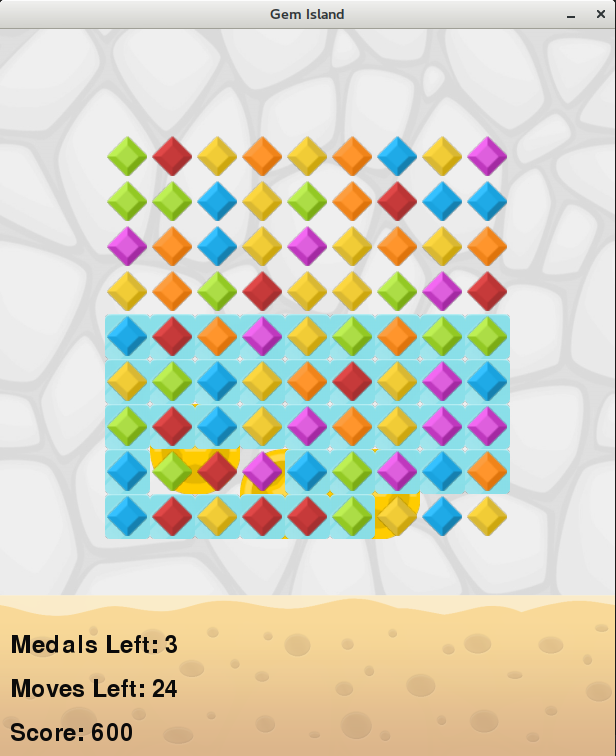
\includegraphics[scale=.3]{media/img/gem_island.png} 
\caption{The match three game: Gem Island}
\label{f.gemisland}
\end{center}
\end{figure}

\section*{Aim}
I will develop policies to play a match three game, two main variants will be made, one will be quicker and allow for more frequent evaluations and another made through deep learning will provide better evaluations but be more complex and slower.


\section*{Plan}

The work I will undertake is outlined in this section. Tasks are further divided into sub-tasks. Also provided is a Gantt chart to show visually how the project will progress. 

\newpage

\begin{table}[]
\centering
\resizebox{\textwidth}{!}{
\begin{tabular}{|p{2.5cm}|p{10.88cm}|}
\hline
Task        &        1. Complete game
\\ \hline
Due        &        13/06/2017
\\ \hline
Objectives        &        To build a challenging game for an AI agent to solve.
\\ \hline
Description        &        \begin{tabular}[c]{@{}p{10.88cm}@{}}1.1 Make a simple game for proof of concept\\ 1.2 Implement matches for gems\\ 1.3 Implement removable ice\\ 1.4 Implement 'gravity' to pull down gems\\ 1.5 Implement animations\\ 1.6 Implement scoring system\\ 1.7 Implement bonus gems\\ 1.8 Implement combination scoring\end{tabular}
\\ \hline
Milestones        &        \begin{tabular}[c]{@{}p{10.88cm}@{}}1.1 Making a simple game\\ 1.6 A fully working game without bonuses\end{tabular}
\\ \hline
Deliverable        &        A complete game for the AI to solve
\\ \hline
\end{tabular}
}
\end{table}


\begin{table}[]
\centering
\resizebox{\textwidth}{!}{
\begin{tabular}{|p{2.5cm}|p{10.88cm}|}
\hline
Task        &        2. Set up game for AI
\\ \hline
Due        &        19/6/2017
\\ \hline
Objectives        &        To get the game in a state for the AI to control.
\\ \hline
Description        &        \begin{tabular}[c]{@{}p{10.88cm}@{}}2.1 Design the game state representation\\ 2.2 Implement methods to get game state\\ 2.3 Implement methods for AI to call\end{tabular}
\\ \hline
Milestones        &        2.3 Game can now be controlled by AI
\\ \hline
Deliverable        &        A game designed so that an AI can control it.
\\ \hline
\end{tabular}
}
\end{table}

\begin{table}[]
\centering
\resizebox{\textwidth}{!}{
\begin{tabular}{|p{2.5cm}|p{10.88cm}|}
\hline
Task        &        3. Build na\"{i}ve AI version 1
\\ \hline
Due        &        22/6/2017
\\ \hline
Objectives        &        Proof of concept for getting an AI to control the game.
\\ \hline
Description        &        \begin{tabular}[c]{@{}p{10.88cm}@{}}3.1 Implement random policy/move selection\\ 3.2 Connect AI to game\\ 3.3 Collate training data from version 1\end{tabular}
\\ \hline
Milestones        &        3.3 Now have data that can be used for training
\\ \hline
Deliverable        &        A working AI which can control the game.
\\ \hline
\end{tabular}
}
\end{table}


\begin{table}[]
\centering
\resizebox{\textwidth}{!}{
\begin{tabular}{|p{2.5cm}|p{10.88cm}|}
\hline
Task        &        4. Build na\"{i}ve AI version 2
\\ \hline
Due        &        28/6/2017
\\ \hline
Objectives        &        Proof of concept for using MCTS, evaluation function, and a policy
\\ \hline
Description        &        \begin{tabular}[c]{@{}p{10.88cm}@{}}4.1 Design search, policy, and evaluation function (s, p, e) \\ 4.2 Implement s, p, e with 1-step look-ahead\\ 4.3 Collate training data from version 2\end{tabular}
\\ \hline
Milestones        &        \\ \hline
Deliverable        &        A na\"{i}ve version of the final design of the AI.
\\ \hline
\end{tabular}
}
\end{table}

\begin{table}[]
\centering
\resizebox{\textwidth}{!}{
\begin{tabular}{|p{2.5cm}|p{10.88cm}|}
\hline
Task        &        5. Gather and collate training data
\\ \hline
Due        &        27/6/2017
\\ \hline
Objectives        &        To obtain the required training data for the neural networks.
\\ \hline
Description        &        \begin{tabular}[c]{@{}p{10.88cm}@{}}5.1 Set up game to output state to file\\ 5.2 Set up game to distribute to users\\ 5.3 Distribute game to users\end{tabular}
\\ \hline
Milestones        &        -
\\ \hline
Deliverable        &        \begin{tabular}[c]{@{}p{10.88cm}@{}}Game to distribute - 22/06/17\\ Collated training data 27/07/17\end{tabular}
\\ \hline
\end{tabular}
}
\end{table}





\begin{table}[]
\centering
\resizebox{\textwidth}{!}{
\begin{tabular}{|p{2.5cm}|p{10.88cm}|}
\hline
Task        &        6. Build Monte Carlo tree search program
\\ \hline
Due        &        21/7/2017
\\ \hline
Objectives        &        To build a tree search program to solve the game.
\\ \hline
Description        &        \begin{tabular}[c]{@{}p{10.88cm}@{}}6.1 Design and implement MCTS program with multi-step look-ahead\\ 6.2 Connect MCTS program to AI\end{tabular}
\\ \hline
Milestones        &        -
\\ \hline
Deliverable        &        A working AI similar in design to AlphaGo
\\ \hline
\end{tabular}
}
\end{table}



\begin{table}[]
\centering
\resizebox{\textwidth}{!}{
\begin{tabular}{|p{2.5cm}|p{10.88cm}|}
\hline
Task        &        7. Build initial policy heuristic using hand chosen features
\\ \hline
Due        &        28/06/2017
\\ \hline
Objectives        &        Build a simple policy that assigns weights the features of different moves
\\ \hline
Description        &        \begin{tabular}[c]{@{}p{10.88cm}@{}} 7.1 Select features to be used \\  7.2 Determine weights of features from training data \\ 7.3 Connect policy to game \end{tabular}
\\ \hline
Milestones        &        -
\\ \hline
Deliverable        &        A basic policy to evaluate actions
\\ \hline
\end{tabular}
}
\end{table}

\begin{table}[]
\centering
\resizebox{\textwidth}{!}{
\begin{tabular}{|p{2.5cm}|p{10.88cm}|}
\hline
Task        &        8. Build policy neural network from whole game state
\\ \hline
Due        &        4/7/2017
\\ \hline
Objectives        &        Build a more complex policy to choose actions
\\ \hline
Description        &        \begin{tabular}[c]{@{}p{10.88cm}@{}} 8.1 Build neural network \\  8.2 Train neural network with training data \\ 8.3 Connect policy network to game \end{tabular}
\\ \hline
Milestones        &        -
\\ \hline
Deliverable        &        A more complex policy to evaluate actions
\\ \hline
\end{tabular}
}
\end{table}

\begin{table}[]
\centering
\resizebox{\textwidth}{!}{
\begin{tabular}{|p{2.5cm}|p{10.88cm}|}
\hline
Task        &        9. Build policy neural network from auto-encoder features
\\ \hline
Due        &        14/07/2017
\\ \hline
Objectives        &        Build a more intelligent policy which will be given the features of interest
\\ \hline
Description        &        \begin{tabular}[c]{@{}p{10.88cm}@{}} 9.1 Build neural network \\  9.2 Train neural network with training data \\ 9.3 Connect policy network to game \\ 9.4 Compare results with those of previous NN \end{tabular}
\\ \hline
Milestones        &        -
\\ \hline
Deliverable        &        A faster complex policy to evaluate actions
\\ \hline
\end{tabular}
}
\end{table}

\begin{table}[]
\centering
\resizebox{\textwidth}{!}{
\begin{tabular}{|p{2.5cm}|p{10.88cm}|}
\hline
Task        &        10. Integration of work with Tom Brereton
\\ \hline
Due        &        21/7/2017
\\ \hline
Objectives        &        Integration of work to build AI which can solve the game.
\\ \hline
Description        &        \begin{tabular}[c]{@{}p{10.88cm}@{}}10.1 Integration of work\end{tabular}
\\ \hline
Milestones        &        -
\\ \hline
Deliverable        &        A working AI similar in design to AlphaGo
\\ \hline
\end{tabular}
}
\end{table}

\begin{table}[]
\centering
\resizebox{\textwidth}{!}{
\begin{tabular}{|p{2.5cm}|p{10.88cm}|}
\hline
Task        &        11. Write dissertation
\\ \hline
Due        &        31/08/2017
\\ \hline
Objectives        &        Write the dissertation for the whole project
\\ \hline
Description        &        \begin{tabular}[c]{@{}p{10.88cm}@{}}  11.1 Complete literature review, 31/06/2017 \\11.1 Draft outline, 06/07/2017  \\  11.3 Problem to be addressed, 10/07/2017 \\ 11.4 Work to be undertaken, 14/07/2017 \\ 11.5 Methodology for simple policy, 25/07/2017 \\ 11.6 Methodology for policy network one, 01/08/2017 \\ 11.7 Methodology for policy network two, 08/08/2017 \\ 11.8 Technical Implementation, 15/08/2017 \\ 11.9 Discussion of results, 22/08/2017 \\ 11.10 Conclusion, 24/08/2017 \\ 11.11 Completing Dissertation, 31/08/2017 \end{tabular}
\\ \hline
Milestones        &        -
\\ \hline
Deliverable        &        Complete dissertation
\\ \hline
\end{tabular}
}
\end{table}

\begin{figure}
\begin{center}
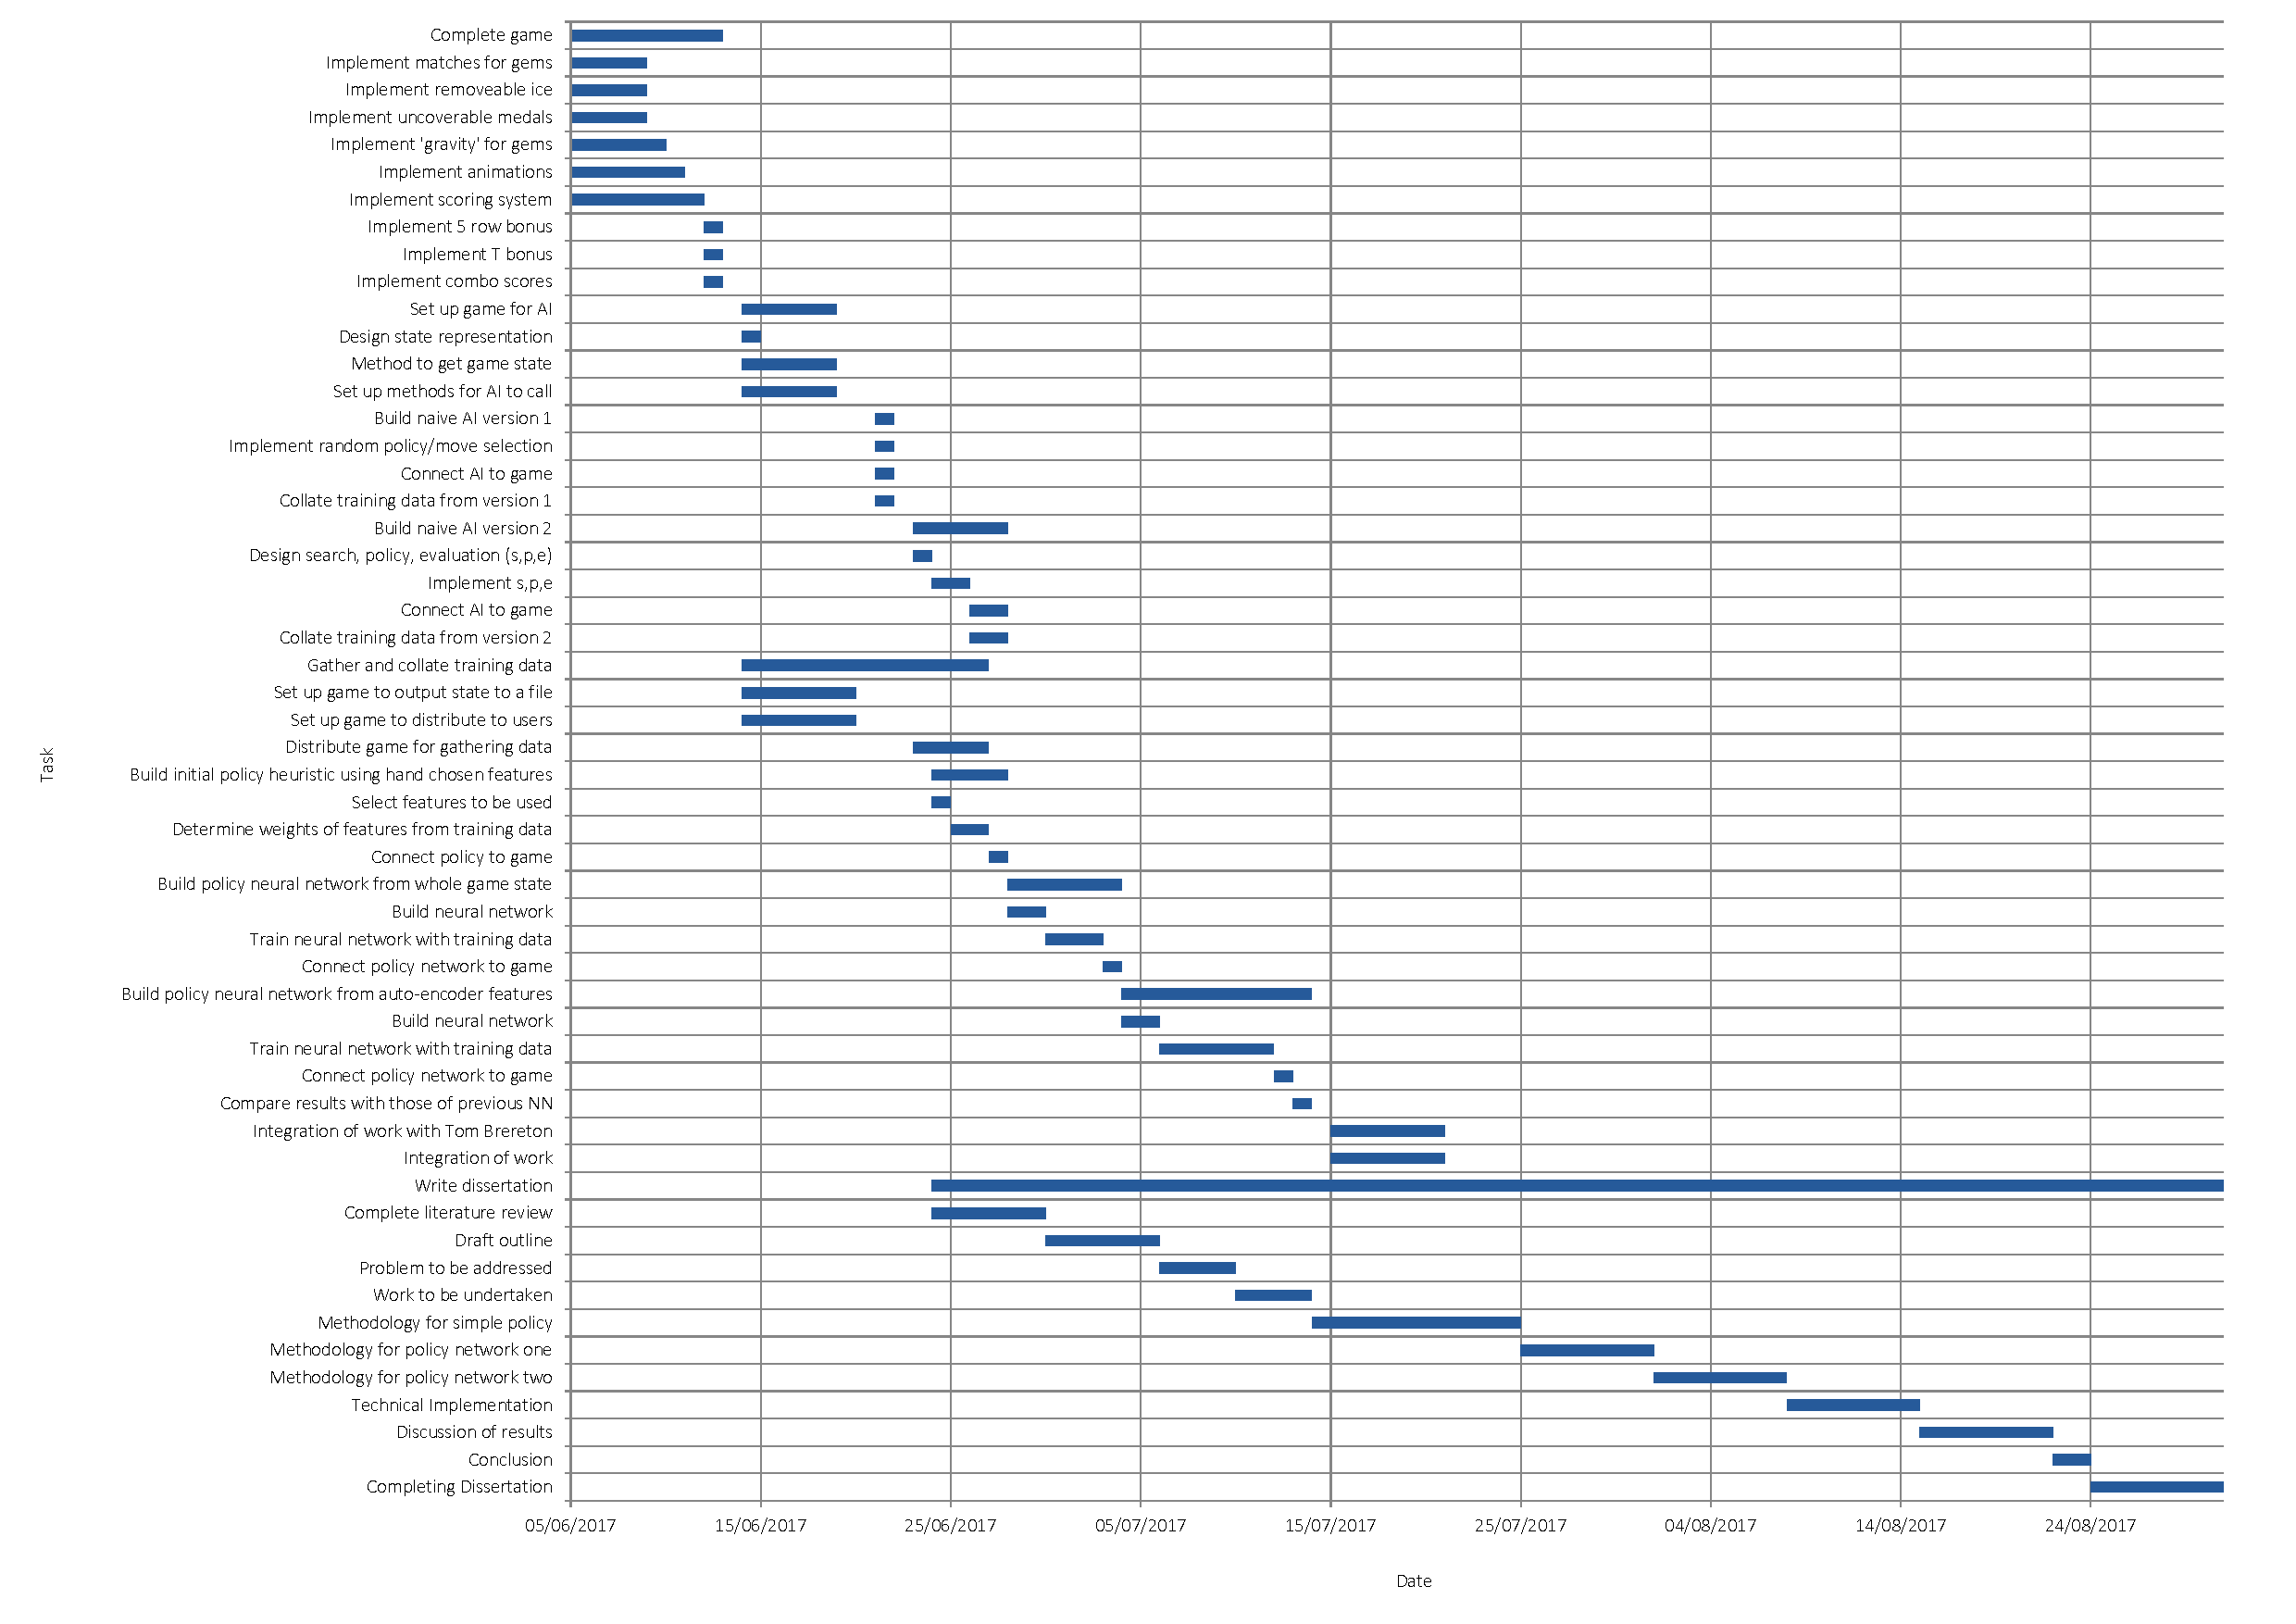
\includegraphics[scale=0.525,origin=c,angle=90]{media/img/GanttChart.pdf} 
\caption{Gantt chart}
\end{center}
\end{figure}

\end{document}